\chapter{規範場、相互作用尺度與帶電弱流}

量子電動力學與量子色動力學在實驗室中的表現看來迥異，但兩者都是規範理論。事實上，標準模型幾乎所有相互作用都以這種方式組織。\emph{規範}一詞有更深的意涵，涉及局域對稱性；這套理論架構可以稍後再談。目前我們只需要最基本的物理描述：規範理論包含類似麥克斯韋理論的場、守恆源、對稱變換、規範玻色子，以及發射和吸收這些玻色子的規則。

\section{作為原型的麥克斯韋理論}

\subsection{場與位勢}

電磁場有六個分量：三個電場分量和三個磁場分量。同一份資訊也可以用一個四維位勢向量來編碼，不過其中帶有一些冗餘：
\begin{equation}
A_\mu=(A_0,\boldsymbol A),
\end{equation}
其中，\(A_0\)是靜電位，\(\boldsymbol A\)是空間向量位勢。在靜電極限下，電場由空間梯度求得：
\begin{equation}
\boldsymbol E=-\boldsymbol\nabla A_0,
\qquad
\boldsymbol F=q\boldsymbol E,
\end{equation}
磁場則為
\begin{equation}
\boldsymbol B=\boldsymbol\nabla\times\boldsymbol A.
\end{equation}
第一個方程的正負號取決於位勢的標準定義；黑板上的討論主要著眼於場是位勢的導數這一點。
\editorialnote{對於隨時間變化的場，完整關係為
\(\boldsymbol E=-\boldsymbol\nabla A_0-\partial_t\boldsymbol A\)。本講在此有意只討論較簡單的靜電情形。}

\begin{figure}[htbp]
\centering
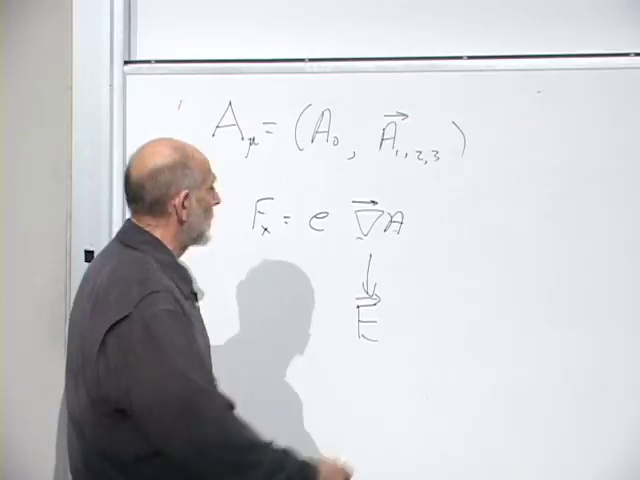
\includegraphics[width=0.62\textwidth]{lecture_05_figure_02.png}
\caption{電磁四維位勢及其與場之間的導數關係。}
\lectureframe{00:03:33}
\end{figure}

因此，電動力學有兩種等價的描述方式：一種以\(\boldsymbol E\)和\(\boldsymbol B\)描述，另一種則以\(A_\mu\)描述。後者只列出四個分量，因為不同的位勢可以描述相同的物理場。這種冗餘是「規範」一詞背後的第一個線索，不過我們暫時還不會正式使用這個概念。

\subsection{波與偏振}

麥克斯韋方程允許波動解。考慮一個沿單位向量\(\hat{\boldsymbol k}\)傳播的平面波。電場和磁場在每一點都與傳播方向垂直：
\begin{equation}
\boldsymbol E\cdot\hat{\boldsymbol k}=0,
\qquad
\boldsymbol B\cdot\hat{\boldsymbol k}=0,
\qquad
\boldsymbol E\cdot\boldsymbol B=0.
\end{equation}
在\(c=1\)的單位制下，兩者的大小相等：
\begin{equation}
|\boldsymbol E|=|\boldsymbol B|.
\end{equation}
對線偏振波而言，\(\boldsymbol E\)的方向決定偏振方向。整個波的形態以光速傳播。

量子化改變了描述方式，卻不改變偏振的結構。電磁波的量子就是光子。把光子畫成一個點難免會造成誤解，但不妨想像這個點帶著一根小小的橫向指針，標示其偏振方向。四分之一波片或其他光學元件可以旋轉偏振方向。靜態庫侖場也可以粗略地想像成由光子反覆發射與吸收所形成。

\subsection{源、通量與守恆}

電磁波可以在真空中傳播，但電磁場也有源：電荷與電流。正點電荷會產生向外的徑向電場，其大小正比於\(1/r^2\)。穿過以該電荷為中心的任意球面的場線數目，不隨球面半徑改變。以數學表示為
\begin{equation}
\oint_{S^2}\boldsymbol E\cdot d\boldsymbol S
=\frac{Q_{\mathrm{enc}}}{\epsilon_0},
\label{eq:l5-gauss}
\end{equation}
其中採用 SI 單位制。

這不只是計算電場的一種方便方法。電場線只能終止於電荷。若一個孤立電荷憑空消失，它的電場就必須同時在所有地方消失，這會違反因果律；或者，缺失電場的前沿必須向外傳播，讓場線終止於空無一物之處。這兩種情況都不允許。因此，通量的幾何性質自然導向電荷守恆：電荷可以移動，正負電荷可以湮滅，但若沒有相應電流補償，淨電荷就不能在局部消失。

相應的局域表述是連續方程：
\begin{equation}
\partial_t\rho+\boldsymbol\nabla\cdot\boldsymbol J=0.
\label{eq:l5-continuity}
\end{equation}
\editorialnote{方程~\eqref{eq:l5-continuity}是課堂上以口頭方式說明的因果性通量論證，所對應的標準局域數學形式。}

\subsection{規範理論的實用定義}

現在可以列出規範理論的基本模式。規範理論具有：
\begin{itemize}
\item 類似電場與磁場的場；
\item 在相互作用夠弱時，表現類似光波的波；
\item 類似電荷的源；
\item 將通量與這些源聯繫起來的高斯定律；
\item 守恆定律及其相關對稱性；
\item 稱為規範玻色子的場量子；以及
\item 控制玻色子發射與吸收的耦合常數。
\end{itemize}
源不一定是電荷。作為一個刻意選取的非物理例子，試想將重子數規範化。質子和中子的重子數都是\(+1\)，因此它們會透過一種新的類庫侖力互相排斥；質子與反質子則會互相吸引。這種理論在數學上可以想像，但自然界中並未觀測到與重子數耦合的長程規範場。單有守恆定律，並不保證存在規範力。

電荷確實伴隨著一種對稱性。對帶電物質場而言，
\begin{equation}
\psi(x)\longmapsto e^{i\theta}\psi(x).
\label{eq:l5-u1}
\end{equation}
相位對稱性與電荷守恆，是同一結構的兩個面向。稍後可以讓\(\theta\)依賴時空位置，藉此看出為什麼需要位勢\(A_\mu\)。在此處，全域變換已足以辨認守恆電荷。

\section{作為非阿貝爾例子的 QCD}

\subsection{三重態、反三重態與膠子矩陣}

在量子色動力學中，夸克場帶有色指標\(i\in\{r,g,b\}\)，並依照\(SU(3)\)的基本表示進行變換：
\begin{equation}
q'_i=U_{ij}q_j,
\qquad
U^\dagger U=\boldsymbol 1,
\qquad
\det U=1.
\label{eq:l5-q-transform}
\end{equation}
這是在三維複數色空間中的旋轉，而不是普通位置空間中的旋轉。這個三分量表示也稱為定義表示。

反粒子場以複共軛變數表示。對式~\eqref{eq:l5-q-transform}取複共軛，可得
\begin{equation}
q_i^{\prime *}=U_{ij}^*q_j^*.
\label{eq:l5-antiquark-transform}
\end{equation}
因此，夸克依照\(\boldsymbol 3\)變換，反夸克則依照\(\bar{\boldsymbol 3}\)變換。

\begin{figure}[htbp]
\centering
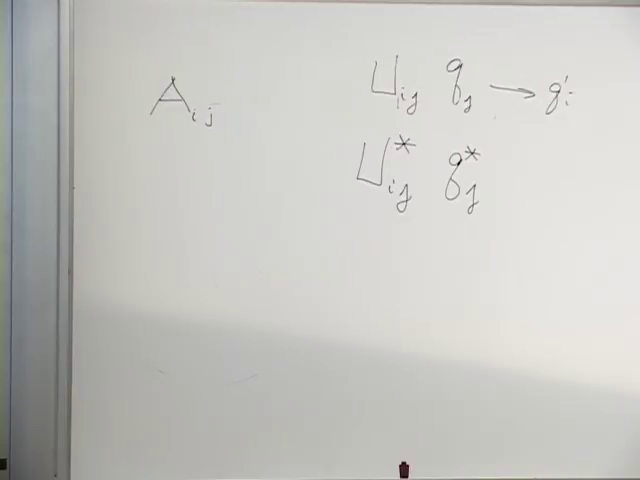
\includegraphics[width=0.62\textwidth]{lecture_05_figure_03.png}
\caption{基本表示的變換及其複共軛的反三重態變換。}
\lectureframe{00:18:47}
\end{figure}

\begin{classroomqa}
\audiencequestion{\(U\)矩陣有幾個？--七個、八個，還是九個？
\lecturetimestamp{00:19:37}}
\lecturerresponse{群元素\(U\)有無限多個。這裡要數的有限數目是獨立生成元的個數；對\(SU(3)\)而言，這個數目是八。一個一般的\(3\times3\)矩陣有九個矩陣元素位置，但特殊么正條件使其只有八個連續自由度。}
\end{classroomqa}

膠子場可以寫成無跡矩陣\(A_{ij}\)。其中一個指標像夸克那樣變換，另一個則像反夸克那樣變換，因此其色結構屬於
\begin{equation}
\boldsymbol 3\otimes\bar{\boldsymbol 3}
=\boldsymbol 1\oplus\boldsymbol 8.
\end{equation}
QCD 保留無跡的八重態：
\begin{equation}
A_{ii}=\operatorname{tr}A=0,
\end{equation}
並排除單態。這就是 QCD 有八種膠子而非九種的原因。更一般而言，\(SU(N)\)有
\begin{equation}
N^2-1
\end{equation}
個生成元，也有同樣數目的規範玻色子場。

光子在電荷\(U(1)\)作用下是中性的：旋轉電子的相位，不會把光子變換成另一種光子。膠子則不同。膠子帶有一個色和一個反色，因此屬於伴隨表示。例如，紅--反藍的組合並非色單態，儘管其中有一個色和一個反色。

\subsection{指標流與自相互作用}

追蹤指標就能讀出相互作用規則。概略而言，色為\(i\)的夸克可以變成色為\(j\)的夸克，同時發射一個帶有相應色流的膠子：
\begin{equation}
q_i\longrightarrow q_j+A_{ij}.
\label{eq:l5-quark-gluon-vertex}
\end{equation}
\(i\)和\(j\)的確切位置取決於箭頭的約定；不變的內容是，進入頂點的每個指標都必須沿著另一條線延續。沒有色指標會消失。

這項規則適用於任何\(SU(N)\)規範理論。基本表示的物質帶有一個指標，反基本表示的物質帶有一個共軛指標，而規範玻色子兩種指標各有一個。物理名稱可以不同，但指標結構不變。

膠子本身帶有色，因此可以發射另一個膠子。一個\(A_{ij}\)膠子可以經由中間指標\(k\)分裂，概略表示為
\begin{equation}
A_{ij}\longrightarrow A_{ik}+A_{kj}.
\label{eq:l5-three-gluon-index}
\end{equation}
這並非完整的楊--米爾斯頂點，但顯示了色流。在普通電動力學中，光子沒有類似的過程。因此膠子會對膠子施力，非阿貝爾場的動力學也比麥克斯韋線性理論複雜得多。

禁閉是其中一項定性的後果。色通量線不能終止，而其自相互作用會將它們拉成連接夸克與反夸克的管狀結構。管中的能量每單位長度大致固定：
\begin{equation}
V(R)\simeq \sigma R.
\end{equation}
因此，把兩端拉得更遠會儲存更多能量，而不是釋放出孤立的色荷。這就是膠子「黏稠」圖像中的關鍵：場本身會阻止帶色的組分以自由粒子形式逃逸。

\section{耦合常數與強弱的意義}

\subsection{電荷作為發射振幅}

規範理論還需要耦合常數。在 QED 中，電子電荷\(e\)是電子--光子頂點的相關係數。它是振幅，而機率是振幅的平方。從操作上來看，可以想像用陰極射線管讓一個高速電子突然停止。電子輻射出光子的機率正比於\(e^2\)；慣例上的因子則併入精細結構常數：
\begin{equation}
\alpha=\frac{e^2}{4\pi\hbar c}
\simeq \frac{1}{137}.
\label{eq:l5-alpha}
\end{equation}
在自然單位制\(\hbar=c=1\)下，耦合是無因次的。若單次基本發射的機率尺度約為百分之一，電磁相互作用在微擾意義下就算弱：大多數被迫停止的電子不會各自放出一簇高能光子。

\subsection{自然單位制連結能量、時間與距離}

令
\begin{equation}
c=1,
\qquad
\hbar=1.
\end{equation}
則時間與距離的單位相同，而能量的單位則是其倒數：
\begin{equation}
E=\hbar\omega\longrightarrow E=\omega\sim\frac1t,
\qquad
x\sim t\sim\frac1E.
\end{equation}
能量越高，所能探測的距離和時間尺度越短。

作為參照，
\begin{equation}
1\ {\rm eV}^{-1}
=\frac{\hbar c}{1\ {\rm eV}}
\simeq 1.97\times10^{-7}\ {\rm m}.
\end{equation}
因此，尺度約為\(10^{-10}\ {\rm m}\)的原子長度，大致相當於千電子伏特的倒數。這些只是數量級換算，並非精密光譜學的結果。

\subsection{原子內部的尺度層級}

以典型原子為例，取
\begin{equation}
R_{\rm atom}\sim10^{-10}\ {\rm m}.
\end{equation}
光穿越這段距離所需的時間為
\begin{equation}
t_{\rm transit}^{\rm atom}\sim10^{-18}\ {\rm s}.
\end{equation}
然而，在輕原子中，電子的速度只有光速的一小部分。依玻爾圖像，\(v/c\sim\alpha\)，因此典型的軌道週期更長：
\begin{equation}
t_{\rm orbit}^{\rm atom}\sim10^{-16}\ {\rm s}.
\end{equation}

激發態原子輻射衰變所需的時間還要更長：
\begin{equation}
t_{\rm decay}^{\rm atom}\sim10^{-9}\ {\rm s}
\end{equation}
這是課堂所用的大略估計。從物理圖像來看，有兩種抑制因素：電磁力所產生的加速度不大，而受加速的電子發射光子的機率也受到\(\alpha\)控制，並且很小。因此，精細結構常數小，使穿越時間、軌道時間與輻射衰變時間之間形成層級差異。

\subsection{強子中沒有這種層級差異}

強子是由夸克和膠子組成、類似原子的束縛系統，但其尺度小得多：
\begin{equation}
R_{\rm hadron}\sim10^{-15}\ {\rm m},
\qquad
t_{\rm transit}^{\rm hadron}\sim10^{-23}\ {\rm s}.
\end{equation}
夸克穿越強子的時間尺度幾乎相同，而會經由強作用衰變的激發態強子，其壽命也大約是
\begin{equation}
t_{\rm orbit}^{\rm hadron}
\sim t_{\rm decay}^{\rm hadron}
\sim10^{-23}\ {\rm s}.
\end{equation}
受撞擊的強子可能會振動並發射一個 {\proseunicodefont π} 介子，所需時間幾乎短到因果律所允許的極限。這裡不像原子內部那樣，存在相差七到九個數量級的時間尺度。

\begin{classroomqa}
\audiencequestion{狹義相對論是否表示，強子的衰變時間不可能顯著短於其光穿越時間？
\lecturetimestamp{00:47:15}}
\lecturerresponse{以數量級來說，這確實是合理的上限描述。強衰變發生得幾乎和系統尺度所允許的一樣快；沒有小耦合或其他大幅抑制因素拖慢它們。}
\end{classroomqa}

因此，相應的強耦合遠大於\(\alpha\)。在一個具代表性的強子尺度上，課堂引用的數值為
\begin{equation}
\alpha_{\rm QCD}\sim0.2,
\end{equation}
比起\(1/137\)更接近 1。這就是較早使用「\emph{強相互作用}」這個名稱的動力學根源。
\editorialnote{QCD 耦合會隨能量尺度而變，因此\(\alpha_s\)並非固定數值。這裡引用的是一個隨尺度而變的示例數值，符合課堂原意。}

\begin{classroomqa}
\audiencequestion{強作用的對應耦合是否就稱為強力常數？
\lecturetimestamp{00:48:17}}
\lecturerresponse{慣例上稱為\(\alpha_{\rm QCD}\)，更常稱為\(\alpha_s\)。電磁耦合通常簡稱\(\alpha\)；若在同一段討論中需要區分兩者，也可以用\(\alpha_{\rm QED}\)。}
\end{classroomqa}

\begin{classroomqa}
\audiencequestion{論文會區分裸電磁耦合與經測量、受到屏蔽的值嗎？
\lecturetimestamp{00:48:38}}
\lecturerresponse{會。通常會區分裸耦合與重整化耦合。真空極化會使有效耦合依測量尺度而變。}
\end{classroomqa}

\section{弱衰變之謎}

弱相互作用因衰變時間極長而得名。弱衰變通常比強衰變慢，有時甚至比原子輻射還慢。最早受到研究的例子是核 {\proseunicodefont β} 衰變。

\subsection{中子 {\proseunicodefont β} 衰變}

自由中子經由下列過程衰變：
\begin{equation}
n\longrightarrow p+e^-+\bar\nu_e.
\label{eq:l5-neutron-decay-intro}
\end{equation}
課堂採用的壽命約為 12 分鐘，和\(10^{-23}\ {\rm s}\)相比長得驚人。這裡的論證不需要用到現代的精密數值。

衰變緩慢的部分原因是運動學限制。大致而言，
\begin{equation}
\begin{aligned}
m_n&\simeq940\ {\rm MeV},
&
m_p&\simeq939\ {\rm MeV},
\\
m_e&\simeq0.5\ {\rm MeV}.
\end{aligned}
\end{equation}
中子的靜止能量只有極小一部分可轉為動能。若中子質量小於末態粒子的靜止質量總和，衰變便不可能發生；若中子質量只比閾值高出極微小的量，可用相空間就會極小，衰變也會很慢。但光靠相空間不足以解釋以分鐘計的壽命。

\subsection{帶電 {\proseunicodefont π} 介子排除了閾值這項解釋}

再考慮
\begin{equation}
\pi^-\longrightarrow e^-+\bar\nu_e
\end{equation}
以及其電荷共軛過程。{\proseunicodefont π} 介子的能量遠高於電子通道的閾值，但其弱衰變壽命仍在奈秒量級，而非強子過程的\(10^{-23}\)秒量級。稍後會談到一個類似的 {\proseunicodefont μ} 子通道。因此，這個謎題源自弱相互作用本身，而不只是中子質量近乎簡併所造成的偶然結果。

\editorialnote{帶電 {\proseunicodefont π} 介子的壽命約為\(26\ {\rm ns}\)，主要衰變通道是\(\pi^-\to\mu^-\bar\nu_\mu\)。電子通道受到螺旋度抑制。課堂先討論電子通道，因為其中粒子的記帳最簡單，接著再回頭討論主要的 {\proseunicodefont μ} 子通道。}

{\proseunicodefont β} 衰變一詞源自歷史上的用法：當時將衰變放出的電子稱為 {\proseunicodefont β} 射線。{\proseunicodefont π} 介子與中子的例子涉及相同的帶電流相互作用，儘管兩者的運動學條件差異很大。

\section{夸克與輕子表}

\subsection{色作用沿垂直方向}

將六種夸克味排列成三組配對的欄：
\begin{equation}
(u,d),\qquad(c,s),\qquad(t,b),
\end{equation}
再把每種夸克的紅、綠、藍三種色分別排在不同列。色作用\(SU(3)\)沿垂直方向進行：它會在上夸克的紅、綠、藍版本之間作變換，也會同時對下、粲、奇異、頂和底夸克進行相同的色變換。它不會把上夸克變成下夸克。

\subsection{弱同位旋作用沿水平方向}

弱對稱性則沿另一個方向作用，會混合下列每一對相鄰粒子：
\begin{equation}
Q_1=\begin{pmatrix}u\\d\end{pmatrix},
\qquad
Q_2=\begin{pmatrix}c\\s\end{pmatrix},
\qquad
Q_3=\begin{pmatrix}t\\b\end{pmatrix}.
\label{eq:l5-quark-doublets}
\end{equation}
上型夸克的電荷為\(+2/3\)，下型夸克的電荷為\(-1/3\)，所以每一對中的電荷相差一個單位。
\editorialnote{講者一度說下夸克的電荷是\(-2/3\)。根據前後的相減關係及後續各個過程，這裡採用標準值\(-1/3\)。}

由於這項對稱性作用於二重態，自然選用的群是\(SU(2)\)。它作用於每個夸克二重態的每一種色態，而不改變色。

還有一列粒子不帶色，因此不與膠子相互作用：輕子。它們另外組成三個二重態：
\begin{equation}
L_e=\begin{pmatrix}\nu_e\\e^-\end{pmatrix},
\qquad
L_\mu=\begin{pmatrix}\nu_\mu\\\mu^-\end{pmatrix},
\qquad
L_\tau=\begin{pmatrix}\nu_\tau\\\tau^-\end{pmatrix}.
\label{eq:l5-lepton-doublets}
\end{equation}
中微子不帶電；電子、{\proseunicodefont μ} 子和 {\proseunicodefont τ} 子的電荷則為\(-1\)。同樣地，每個二重態中的兩個成員電荷相差一個單位。電子、{\proseunicodefont μ} 子和 {\proseunicodefont τ} 子具有相同的規範量子數，但質量各不相同；三代上型夸克或下型夸克也有相同的電荷模式。

\begin{figure}[htbp]
\centering
\includegraphics[width=0.82\textwidth]{lecture_05_figure_05.png}
\caption{黑板上的表格：色作用連結紅、藍、綠各列；弱\(SU(2)\)則連結成對的味道欄，以及輕子列。}
\lectureframe{01:03:35}
\end{figure}

在此處把輕子稱為第四種色，只是一種類比。它們在弱同位旋二重態表中佔據第四列，但普通的 QCD \(SU(3)\)不會把夸克變換成輕子。

\section{建構帶電弱玻色子}

\subsection{帶電玻色子的量子數}

規範玻色子具有所需的變換性質，能將二重態的一個成員轉變為另一個。先看輕子對\(e^-\bar\nu_e\)。其電荷為\(-1\)，因此相應的帶電規範玻色子稱為\(W^-\)：
\begin{equation}
W^-\sim e^-\bar\nu_e.
\end{equation}
下夸克與反上夸克也有相同的量子數：
\begin{equation}
W^-\sim d\bar u.
\end{equation}
符號\(\sim\)表示兩者具有相同的相關規範量子數，並不表示\(W\)字面上是由這些粒子束縛而成。其反粒子由共軛組合構成：
\begin{equation}
W^+\sim e^+\nu_e\sim\bar d u.
\end{equation}

帶電弱頂點包括
\begin{align}
e^-&\longrightarrow\nu_e+W^-,
&
\mu^-&\longrightarrow\nu_\mu+W^-,
\label{eq:l5-lepton-w}\\
d&\longrightarrow u+W^-,
&
s&\longrightarrow c+W^-,
\label{eq:l5-quark-w}
\end{align}
運動學條件允許時，第三代粒子也有類似的躍遷。規範玻色子在動力學上實現了與對稱性作用於二重態時相同的水平混合。

\begin{classroomqa}
\audiencequestion{電荷守恆要求放出的玻色子電荷為\(-1\)，但為什麼電子、下夸克和奇異夸克的躍遷都涉及同一種粒子？
\lecturetimestamp{01:12:56}}
\lecturerresponse{這是由共同的弱對稱性所反映的一項實驗事實。自然界完全可以自洽地為每個世代，或分別為夸克與輕子，指定不同的\(W\)型玻色子。但實際上，一個\(SU(2)\)同時作用於所有二重態，而所有這些躍遷都由相同的帶電規範玻色子媒介。}
\end{classroomqa}

\subsection{讀取與反轉頂點}

一個頂點代表一系列過程。將入射線反轉為出射線，會使粒子變成其反粒子；將\(W^-\)線反轉，則會得到\(W^+\)。因此，只要一致地追蹤電荷、動量及所有相關量子數，同一頂點可以描述發射、吸收、衰變、湮滅或其逆反應。

\begin{classroomqa}
\audiencequestion{這些弱頂點中的箭頭和線可以反向嗎？
\lecturetimestamp{01:14:51}}
\lecturerresponse{可以。線可以由末態交叉至初態，或由初態交叉至末態；但如此一來，粒子就會變成其反粒子。因此，同一個局域頂點可以描述許多方向不同的反應。}
\end{classroomqa}

\begin{classroomqa}
\audiencequestion{把奇異夸克線和粲夸克線畫進\(W^-\)，是否表示這個玻色子字面上是由奇異夸克和反粲夸克束縛而成？
\lecturetimestamp{01:15:43}}
\lecturerresponse{不是。線的記帳只表示\(W^-\)承載了這些欄位之間的量子數變化。若把圖讀作衰變，能量足夠高的\(W^-\)可以產生一個奇異夸克和一個反粲夸克；它本身並不是由這兩者組成。}
\end{classroomqa}

\begin{classroomqa}
\audiencequestion{電子和反中微子能否形成\(W\)，再由它產生一對夸克？
\lecturetimestamp{01:17:22}}
\lecturerresponse{正是如此。只要質心能量足夠，初態輕子便能形成帶電流中間態，而這個中間態可以透過允許的夸克通道出現。這兩個頂點和衰變過程中的頂點相同，只是從另一個方向來讀。}
\end{classroomqa}

\subsection{缺少的第三種玻色子}

\(SU(2)\)群有三個生成元，因此有三個規範場。目前只列出了\(W^+\)和\(W^-\)。第三個電中性場必須對應於一些對角組合，例如電子--正電子以及中微子--反中微子的量子數組合。這個場刻意暫置於背景中。它與物理的\(Z\)玻色子及光子的關係，則要等到討論電弱混合時才會說明。

\begin{classroomqa}
\audiencequestion{弱作用和強作用是在不同的歷史時期才受到懷疑的嗎？
\lecturetimestamp{01:24:11}}
\lecturerresponse{兩者的實驗起源都可追溯至早期放射性研究。{\proseunicodefont α} 衰變揭示了核物理與強相互作用，{\proseunicodefont β} 衰變揭示了弱相互作用，而 {\proseunicodefont γ} 衰變則放出電磁光子。早在貝克勒爾的年代，這三項線索就已經全數出現，遠早於現代場論的建立。}
\end{classroomqa}

\section{帶電流衰變範例}

\subsection{{\proseunicodefont π} 介子衰變}

帶負電 {\proseunicodefont π} 介子的價夸克組成為
\begin{equation}
\pi^-=d\bar u.
\end{equation}
這些量子數可以透過湮滅形成\(W^-\)，再由它產生一個帶電輕子及相應的反中微子：
\begin{align}
\pi^-&\longrightarrow W^{-*}
\longrightarrow e^-+\bar\nu_e,
\label{eq:l5-pion-electron}\\
\pi^-&\longrightarrow W^{-*}
\longrightarrow \mu^-+\bar\nu_\mu.
\label{eq:l5-pion-muon}
\end{align}
星號表示中間的\(W\)是虛粒子。第二個通道是主要衰變通道。

\begin{figure}[htbp]
\centering
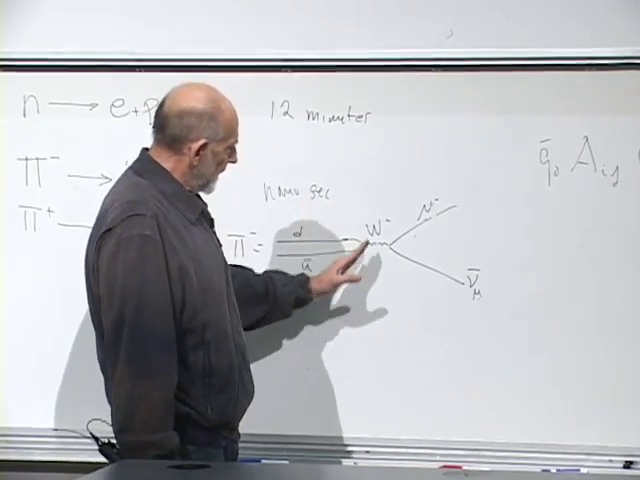
\includegraphics[width=0.72\textwidth]{lecture_05_figure_04.png}
\caption{一個\(d\bar u\){\proseunicodefont π} 介子湮滅形成虛\(W^-\)，接著產生一個帶電輕子及其相應的反中微子。}
\lectureframe{01:19:38}
\end{figure}

\begin{classroomqa}
\audiencequestion{時間方向畫成水平而非垂直，這樣仍算是費曼圖嗎？
\lecturetimestamp{01:20:21}}
\lecturerresponse{算。時間軸在紙面上的方向只是一種約定。只要先指定一個方向代表時間，並一致地解讀所有箭頭，這張圖所表達的相互作用資訊就相同。}
\end{classroomqa}

\begin{classroomqa}
\audiencequestion{這張圖能不能像可逆化學反應那樣來解讀，而不是看成單向、不可逆的衰變？
\lecturetimestamp{01:21:35}}
\lecturerresponse{逆過程是允許的。在真空中產生的 {\proseunicodefont π} 介子會衰變，是因為出射粒子彼此分離，通常不會重新結合。但若讓 {\proseunicodefont μ} 子和反中微子以適當的能量與動量一同撞入，經由反向相互作用形成 {\proseunicodefont π} 介子的振幅便不為零。}
\end{classroomqa}

\subsection{能量與虛中間態}

對於靜止的 {\proseunicodefont π} 介子，
\begin{equation}
m_\pi\simeq140\ {\rm MeV},
\qquad
m_\mu\simeq106\ {\rm MeV},
\qquad
m_\nu\approx0
\end{equation}
在此處所需的精度下，這些數值近似成立。剩餘能量會轉為出射粒子的動能。動量守恆要求
\begin{equation}
\boldsymbol p_\mu+\boldsymbol p_{\bar\nu}=0,
\end{equation}
因此，兩個粒子在 {\proseunicodefont π} 介子的靜止參考系中背向飛離。

\begin{classroomqa}
\audiencequestion{中間態\(W\)的質量遠大於 {\proseunicodefont π} 介子，能量怎麼可能守恆？
\lecturetimestamp{01:25:08}}
\lecturerresponse{只有初態和末態粒子必須位於質量殼上。四動量在每個頂點都守恆，但內部虛線不必滿足\(E^2=\boldsymbol p^2+m_W^2\)。離殼偏差越大，其傳播子對過程的抑制就越強。\editorialnote{講座使用了傳統的能量--時間不確定性說法，並表示中間態可以短暫違反能量守恆。更精確的現代表述如回答所述：能量—動量守恆，但內部虛線不必滿足實粒子的質量殼條件。}}
\end{classroomqa}

\subsection{{\proseunicodefont μ} 子衰變}

{\proseunicodefont μ} 子可以先放出一個虛\(W^-\)，轉變成其對應的中微子：
\begin{equation}
\mu^-\longrightarrow\nu_\mu+W^{-*}.
\end{equation}
接著，這個虛玻色子會產生一個電子和一個電子反中微子：
\begin{equation}
\mu^-\longrightarrow
\nu_\mu+e^-+\bar\nu_e.
\label{eq:l5-muon-decay}
\end{equation}
這是純輕子過程。{\proseunicodefont μ} 子的質量約為電子的 200 倍，因此末態粒子的靜止質量之外，還有充足能量可轉化為動能。

\begin{figure}[htbp]
\centering
\includegraphics[width=0.72\textwidth]{lecture_05_figure_06.png}
\caption{{\proseunicodefont μ} 子經由虛帶電弱玻色子衰變。}
\lectureframe{01:29:24}
\end{figure}

\begin{classroomqa}
\audiencequestion{與電子一同發射的中性粒子是反中微子嗎？
\lecturetimestamp{01:29:06}}
\lecturerresponse{是的。完整的末態包含一個 {\proseunicodefont μ} 中微子、一個電子反中微子和一個電子。保留味標籤，就能避免混淆這兩個中性粒子。}
\end{classroomqa}

電子在真空中無法逆向進行這個衰變，因為電子比 {\proseunicodefont μ} 子輕。{\proseunicodefont τ} 子較重，可以經由類似的弱作用通道衰變。這裡的穩定性部分只是質量排序所造成的偶然結果，並非底層頂點有所不同。

\begin{classroomqa}
\audiencequestion{直線加速器是否等於有效地增加電子的質量，讓原本禁戒的反應得以反向進行？
\lecturetimestamp{01:30:23}}
\lecturerresponse{它不會改變電子的不變靜止質量，而是提供動能。足夠的質心能量可以產生較重的末態粒子；因此，只要將質量改成可用的碰撞能量，這個物理想法就是正確的。}
\end{classroomqa}

\subsection{夸克層次的中子 {\proseunicodefont β} 衰變}

中子和質子的價夸克組成如下：
\begin{equation}
n=udd,
\qquad
p=uud.
\end{equation}
中子中的一個下夸克經歷帶電流躍遷：
\begin{equation}
d\longrightarrow u+W^{-*},
\end{equation}
使 \(udd\) 轉變為 \(uud\)。接著，虛玻色子衰變為：
\begin{equation}
W^{-*}\longrightarrow e^-+\bar\nu_e.
\end{equation}
將這兩個頂點結合起來，就會得到
\begin{equation}
n\longrightarrow p+e^-+\bar\nu_e.
\end{equation}

相反的夸克躍遷 \(u\to d+W^+\) 會留下由三個下夸克組成的重子，但這個可達到的末態對自由中子而言太重，無法產生。實際發生的下夸克轉變為上夸克，才是能量上允許的路徑。

\begin{classroomqa}
\audiencequestion{中子能不能改為衰變成一個質子、一個 {\proseunicodefont μ} 子和相應的反中微子？
\lecturetimestamp{01:32:38}}
\lecturerresponse{對於靜止的自由中子而言，不能：中子--質子的質量差遠小於 {\proseunicodefont μ} 子的質量。若有足夠的額外碰撞能量或激發能量，同一個弱作用頂點也能參與產生 {\proseunicodefont μ} 子的反應通道。這是運動學上的禁戒，並非缺少相互作用。}
\end{classroomqa}

\section{尚未解開的壓低之謎}

帶電弱作用頂點說明了哪些過程可以發生，卻還沒有解釋它們為何如此緩慢。一個看似合理的答案是弱耦合極其微小，但這個答案不對：無因次的弱規範耦合大小大致與電磁耦合相當。這種壓低必定另有原因。

虛傳播子已顯示出缺少的關鍵：\(W\)的質量非常大。在遠低於 \(m_W\) 的能量下，帶電流振幅會受到大致與 \(1/m_W^2\) 的冪次成比例的壓低。待希格斯機制和電弱對稱性破缺說明規範玻色子如何獲得質量後，我們再來展開這個關聯。
\editorialnote{講座將這個問題留待下一次課程討論。此處納入重 \(W\) 的解釋，是為了預先連結後續內容，並非表示這項推導已在本講座中完成。}

\begin{classroomqa}
\audiencequestion{我們說這個理論具有這種對稱性，是指它的拉格朗日量在相應的變換下保持不變嗎？
\lecturetimestamp{01:34:14}}
\lecturerresponse{正是如此。說這個理論具有該對稱性，是指拉格朗日量，或等價地說，作用量在這些變換下保持不變。完整的拉格朗日量只是留待之後寫出，並非改用其他定義。}
\end{classroomqa}

這條脈絡至此已完整：麥克斯威理論提供原型；QCD 展示非阿貝爾規範玻色子如何攜帶並交換荷；耦合常數說明原子與強子的時間尺度為何不同；而弱 \(SU(2)\) 則將夸克和輕子組成由 \(W^\pm\) 相連的二重態。接下來要理解的是，為什麼這些由規範作用中介的過程在實際上如此微弱，儘管其底層耦合並不特別小。